\documentclass{tufte-handout}

\title{Leafleting Effectiveness Survey (LES)}
\author[Jack Norris \& Eric Roberts \& Jonathon Smith]{Jack Norris\thanks{Executive Director, Vegan Outreach (jack@veganoutreach.org), \textit{LES Roles:} Study Lead, Logistics, Reporting } \& Eric Roberts\thanks{Research Manager, California Department of Health Services (trax11@16mail.com), \textit{LES Roles:} Statistical Analyst} \& Jonathon Smith\thanks{Technical Group Supervisor, Jet Propulsion Laboratory (jonathon.j.smith@gmail.com), \textit{LES Roles:} Consultant}}

\date{June 2017} % without \date command, current date is supplied
%\geometry{showframe} % display margins for debugging page layout

\usepackage{graphicx} % allow embedded images
  \setkeys{Gin}{width=\linewidth,totalheight=\textheight,keepaspectratio}
  \graphicspath{{graphics/}} % set of paths to search for images
\usepackage{amsmath}  % extended mathematics
\usepackage{booktabs} % book-quality tables
\usepackage{units}    % non-stacked fractions and better unit spacing
\usepackage{multicol} % multiple column layout facilities
\usepackage{colortbl}   % filler text
\usepackage{fancyvrb} % extended verbatim environments
\usepackage[export]{adjustbox}
\usepackage{pdfpages}

  \fvset{fontsize=\normalsize}% default font size for fancy-verbatim environments

% Standardize command font styles and environments
\newcommand{\doccmd}[1]{\texttt{\textbackslash#1}}% command name -- adds backslash automatically
\newcommand{\docopt}[1]{\ensuremath{\langle}\textrm{\textit{#1}}\ensuremath{\rangle}}% optional command argument
\newcommand{\docarg}[1]{\textrm{\textit{#1}}}% (required) command argument
\newcommand{\docenv}[1]{\textsf{#1}}% environment name
\newcommand{\docpkg}[1]{\texttt{#1}}% package name
\newcommand{\doccls}[1]{\texttt{#1}}% document class name
\newcommand{\docclsopt}[1]{\texttt{#1}}% document class option name
\newenvironment{docspec}{\begin{quote}\noindent}{\end{quote}}% command specification environment

\newcommand{\les}[0]{\textsc{LES}}% document class option name


\newcommand{\totalbooklets}[0]{\textsc{65000}}
\newcommand{\giftcardnum}[0]{\textsc{3250.0}}                                   
\newcommand{\schoolnum}[0]{\textsc{32.5}}
\newcommand{\giftcardcost}[0]{\textsc{48750.0}}
\newcommand{\stickercost}[0]{\textsc{9750.0}}                  
\newcommand{\totalrequest}[0]{\textsc{58500.0}} 
\newcommand{\totalvo}[0]{\textsc{12512.5}}              


\begin{document}

\maketitle% this prints the handout title, author, and date


% ---------------------------------------
% ---------------------------------------
\begin{abstract}
\noindent

Near the beginning of Fall semester 2017, a total of \totalbooklets~ 
students will be handed a leaflet with a pro animal rights message 
(\textbf{test books}). Each booklet will have a
sticker advertising a ``\$5 Starbucks or Amazon Gift Card for taking
brief survey" (\textbf{Part 1 Survey}). Students answering the survey will be 
asked about their current consumption of animal products (\textbf{base rate}) 
and given a gift card. One month later, these same students will receive an 
email, "Thanks for taking our previous survey! We have a few more questions, 
of course for another \$10 gift card!" (\textbf{Part 2 Survey}). Students 
will again be asked about their current animal consumption. The data will
be examined to see if the pro-animal leaflets reduce the amount of
animal products consumed by the students (\textbf{post-test rate}), 
particularly to zero (the \textbf{``One Week Vegan"}). 

\end{abstract}

\begin{marginfigure}[0 in]%
  \raggedleft
  
\includegraphics[width=\textwidth]{vologo.png}
  \caption{Vegan Outreach was founded in 1993 and has since handed out more
  than 30 million pro-vegetarian leaflets. They are the organization leading 
  the proposed LES Study.}
  \label{fig:vologo}
\end{marginfigure}
  
\newthought{The Leafleting Effectiveness Survey (\les)} will attempt
to quantify the impact of pro-animal leafleting on the later 
consumption of animal products. In particular it will look for 
``one week vegans", or leaflet recipients who report no consumption of animal 
products in the post-test survey week. The relationship between leafleting 
and one week vegans is of real concern for the organization 
leading \les, Vegan Outreach (VO). VO's primary intervention on behalf of 
animals is to hand out pro-vegetarian, anti-speciest literature to 
college students. Verifying the impact of this intervention has become 
an organizational priority at the highest level. VO also understands that 
this is a general concern of the broader animal protection community, and 
has sought the support and advice of partner organizations to carry out \les.

\begin{fullwidth}
{
\fontsize{9pt}{9pt}\selectfont
\vskip 1.5em
\noindent
\textsc{\les~ At A Glance}
\noindent
\begin{itemize}
    \item[] Utilizes a pre- and post- survey to measure the 
            impact of leafleting on self-reported animal product 
            consumption.
    \item[] Pilot studies indicate that a brightly colored sticker 
            attached to leaflets advertising an incentivized survey
            (\$5 for P1, \$10 for P2, \$15 total per participant) can 
            generate a response rate of roughly 5\%.
    \item[] A total of \totalbooklets~ will be handed out, enabling the 
            study to detect a conversion of approximately 1.5\% or 
            greater of the test population into a one week vegan with
            80\% power.
    \item[] The leaflets will be handed out at \schoolnum~ schools in
            September 2017. Recipients have one week after the leaflets
            are handed out to complete the Part 1 survey. An email will
            be sent out to students who completed Part 1 in 
            mid-October, inviting them to fill out the Part 2 survey.
\end{itemize}
}
\end{fullwidth}

\vskip 1.5em
\noindent
In particular, VO seeking the participation of Animal Charity 
Evaluators (ACE) as a partner on \les. This document outlines VO's formal
request for a grant from ACE's Animal Advocacy Research Fund. VO is 
looking to ACE to finance (1) the printing of \totalbooklets~ 
survey-advertising stickers (\$\stickercost), and (2) the purchase of
\giftcardnum~ gift cards to distribute as incentives for taking the 
survery (\$\giftcardcost). This brings the total amount
of money requested for the study to \textbf{\$\totalrequest}.

An overview of the study design is provided below, and elaborated 
on in more length throughout the rest of the document.


% ---------------------------------------
% ---------------------------------------
\section{Background}\label{sec:background}

\newthought{There have been} a number of previous attempts to measure the 
effectiveness of leafleting (summarized below). These studies have helped 
characterize this largely unexplored landscape, however none of them were 
designed or powered appropriately to answer the question of whether 
leafleting college campuses produces vegans at a reliable rate. 
 
\begin{fullwidth}
{
\fontsize{9pt}{9pt}\selectfont
\vskip 1.5em
\noindent
\textsc{Previous Leafleting Studies}
\noindent
\begin{itemize}
    \item[] In the fall of 2012, Farm Sanctuary and The Humane League partnered 
    in evaluating the impact of leafleting at the University of Delaware and 
    the University of Maryland by surveying 403 students who had received a 
    Vegan Outreach leaflet during their college career With corrected arithmetic, 
    \textbf{1.7 percent} of the recipients said they went vegetarian as a result 
    of the leaflet. Limitations included the absence of a control group comparison, 
    regression analysis, and analysis of statistical significance.
    \item[] In the fall of 2013, Animal Charity Evaluators coordinated a similar 
    study, again using Vegan Outreach leaflets with students from ten American 
    colleges and one Canadian college.The sample sizes were 123 and 477 for the 
    treatment group and the control group respectively. Using a generalized linear 
    model and a chi-square test, the differences in change in consumption of red 
    meat and poultry (but not fish) between the experimental group and the control 
    group were statistically significant at the 99 percent confidence level. 
    Limitations include the absence of a large sample size for each school, 
    and a heavy dependence on the subjects? recollection of their diet three 
    months prior to the survey.
\end{itemize}
}
\end{fullwidth}

Beyond this literature, Vegan Outreach has run a total of three pilot studies
in preparation for a full-scale LES. These pilots have focused primarily on 
crafting an approach that results in a sufficiently high survey response rate to
make a fully powered LES tractable. The current study design (brightly colored stickers 
and \$15 incentive for 5\% response rate) is a direct result of these studies, summarized 
below.  

\begin{marginfigure}[0 in]%
  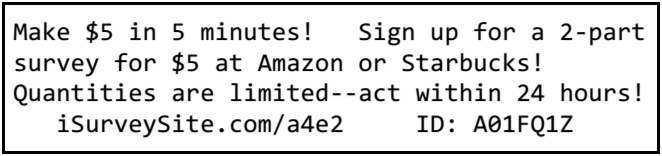
\includegraphics[width=\textwidth]{les_sticker_1.png}\\
  
\includegraphics[width=.98\textwidth]{les_sticker_2.png}
  \caption{Stickers used to adeverstise incentivised surves, pilot 1 and 2 (top), pilot 3 (bottom).}
  \label{fig:lesstickers}
\end{marginfigure}

%\begin{fullwidth}
{  
\fontsize{9pt}{9pt}\selectfont
\vskip 1.5em
\noindent
\textsc{LES Pilot Studies}
\vskip 1em
\noindent
Pilot 1: Fall 2015 
\begin{itemize}
  \item[] The first pilot study utilized a test group of 5000 and a control 
  group of 1000. It used plain white stickers (Figure \ref{fig:lesstickers}) 
  to advertised a \$5 incentivized survey, and achieved an overall response 
  rate of 1.88\%. 
\end{itemize}
\noindent 
Pilot 2: Spring 2016 
\begin{itemize}
  \item[] The second pilot used two separate tests groups, each with 100 
  participants, and no control group. Plain white stickers advertised \$10 
  (group 1) and \$20 (group 2) incentivized surveys and achieved response 
  rates were 3\% and 2\% respectively. 
\end{itemize}
Pilot 3: Spring 2016 
\begin{itemize}
  \item[] The third pilot used a single test group with 600 participants 
  (no control). This time colored stickers (Figure \ref{fig:lesstickers}) 
  advertised a \$5 incentivized survey, and an additional \$10 was offered 
  to complete Part 2 of the survey for a response rate of 5\%. 
\end{itemize}
\vskip 1.5em
}
%\end{fullwidth}

The full-scale LES will use the strategy from Pilot 3. The key elements are
(1) colored stickers, (2) \$5 incentive for Part 1 survey, (3) \$10 for Part 2
survey. 

\begin{marginfigure}[1 in]%
  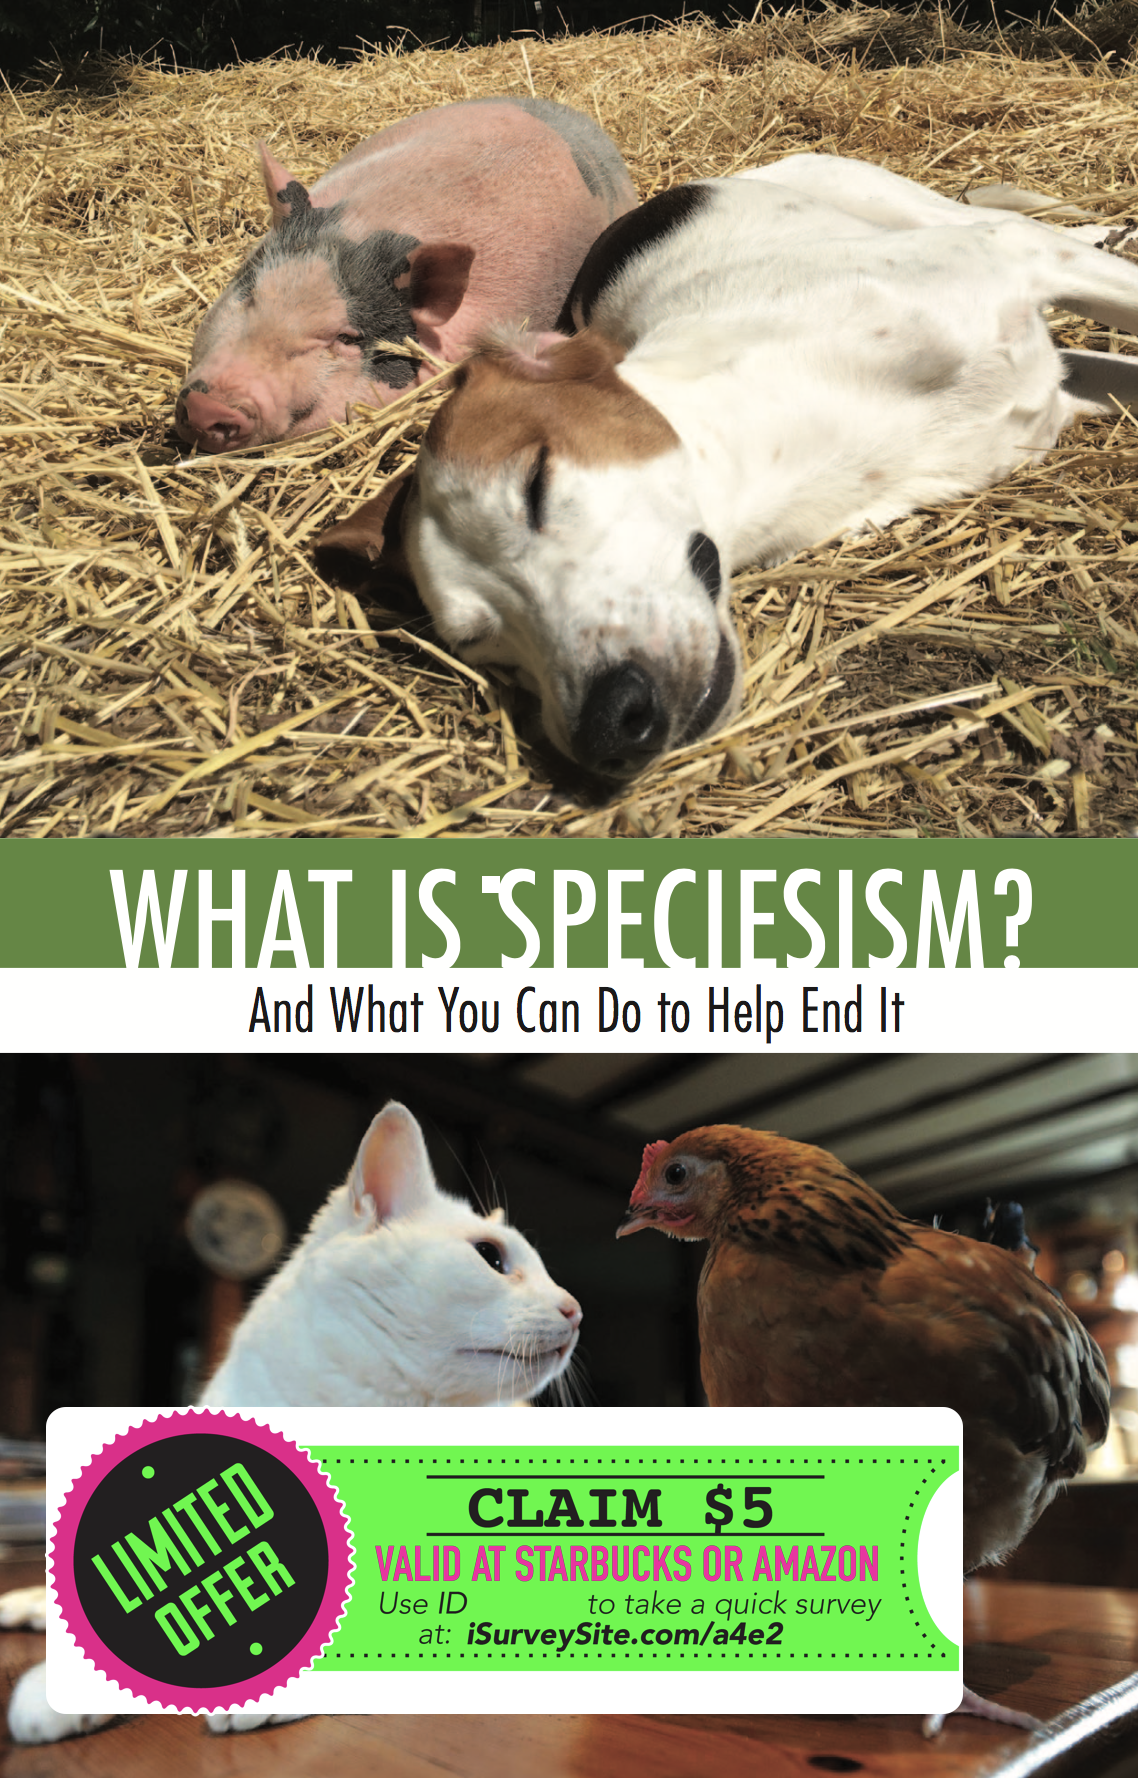
\includegraphics[width=\textwidth]{les_booklet_mockup.png}
  \caption{Mockup of test booklet with survey sticker.}
  \label{fig:lesbooklet}
\end{marginfigure}

% ---------------------------------------
% ---------------------------------------
\section{Methods}

\textit{Note: A detailed description of the study methodology is provided
in the Appendix named ``Study Design and Power Considerations."}

\newthought{The motivation of this study} is to quantify the effect of a leafleting
as an intervention. It uses a pre-test / post-test design where each participant 
is evaluated before and after the intervention. Because each subject's 
covariates are identical both before and after the intervention, comparison 
of pre and post test outcomes becomes relatively straightforward. 
Each participant effectively serves as their own control, except for the
confounding influence of time, which will be addressed later. 

Both pre-test and post-test surveys will include diet frequency questions 
asking subjects to quantify their consumption of various foods during the 
previous week, with response options presented as Likert scales.\footnote{An example
of the survey can be examined at iSurveySite.com} To maximize both statistical 
validity and measurement reliability, outcomes will be analyzed as the 
percent of subjects consuming non-vegan foods less than once per week or 
never (binary variable). Such subject are termed ``one-week vegans" (OWV), and 
measuring the number of OMV's created as the result of leafleting 
is the prime goal of this study.\footnote{The study will also examine the
number of people reporting no beef consumption (``one-week beef avoiders" (OWBA)) 
and no meat consumption of any kind except fish (``one-week pescatarians" (OWP)).}

The study will employ two treatment arms using two different leaflets. This is
in part to make sure that a single, low-performing leaflet doesn't sway the 
overall results of the study. These treatment groups will be pooled when 
when analyzing the survey results for OMVs. The number of subjects
required for the treatment arms depends on the quantities described in Table
\ref{tab:drivers}.

\begin{table*}
  \fontfamily{ppl}\selectfont
  \begin{tabular}{p{2cm}p{7cm}p{6cm}}
    \toprule
    Quantity  & What this is & Reason this is important \\
    \midrule
    Pre-test probability  & How common the outcome is at baseline (that is, prior to the intervention) & The more rare a phenomenon, the more subjects needed to quantify its frequency, or changes in its frequency due to the intervention\\                
    \midrule
    Expected odds ratio  & How much of an effect the intervention is anticipated to have on the outcome & Small effects require more subjects to observe compared to large effects\\                
    \bottomrule
  \end{tabular}
  \vskip 1.5em
  \caption{\les~ Statistical Drivers}
  \label{tab:drivers}
\end{table*}

Table \ref{tab:power} shows the assumed pre-test probabilities and expected 
odds ratios that were used to size the treatment group. These are largely
based on the results of the \les Pilot Studies mentioned above, as well
as ``Pay-Per Read" (PPR) studies undertaken by VO.\footnote{The PPR studies used
Amazon's Mechanical Turk platform to enlist people to read leaflets and 
fill out surveys afterward.}

\vskip 1.5em
\begin{table*}
  \fontfamily{ppl}\selectfont
  \begin{tabular}{p{2cm}p{3cm}p{3cm}p{3cm}p{4 cm}}
    \toprule
    Group  & Pre-test Rate & Expected ratio & \# for 80\% power & \# leaflets to distribute \\
    \midrule
    OWV  & 2.5\% & 1.5 & 3190 & 63800 \\                
    OWBA  & 37.5\% & 1.6 & 200 & 6000 \\                
    OWP  & 2.9\% & 1.7 & 1540 & 30800 \\                
    \bottomrule
  \end{tabular}
  \vskip 1.5em
  \caption{\les~ Power Calculation Assumptions}
  \label{tab:power}
\end{table*}

\subsection*{Control group}

For this design, the potential confounder is time; that is, 
if students are rapidly becoming vegan independently of the 
leaflets, this effect could be misattributed to the intervention.
This is the argument for a separate control group, which would 
undergo the same pre-test and post-test measurements as the 
treatment groups but would receive a spurious intervention 
(that is, a leaflet unrelated to veganism) in between.  

The inclusion of an equal sized control group will roughly double 
the cost of the study by roughly, increasing the amount requested
from ACE to \$117000. If ACE is willing to provide these additional 
funds, a full control group will be utilized for the study. If not, 
than a series of mitigating actions will be employed to minimize 
the impact of time on the study. 

{  
\fontsize{9pt}{9pt}\selectfont
\vskip 1.5em
\noindent
\textsc{Time-variable mitigation measures}
\vskip 1em
\noindent
Shorten pre-post test span 
\begin{itemize}
  \item[] The nominal time span between administering the pre and post
  test surveys is two months (this was used in the pilots). For an 
  uncontrolled study, this will be shortened to one month to minimize
  the opportunity for non-study parmaeters to influence the results. 
\end{itemize}
\noindent 
Minimize other campus outreach activities
\begin{itemize}
  \item[] VO will engage with other players in the AR community and
  ask that they impose a moratorium on campus outreach activities for
  the duration of the study. 
\end{itemize}
\vskip 1.5em
}

% ---------------------------------------
% ---------------------------------------
\section{Plan and Budget}

\newthought{VO will lead} the execution of the study. This will
include printing and stickering the test booklets (and possibly control booklets)
and shipping them to its distributed network of outreach coordinators (OC).
The OCs will hand out the leaflets over a two week period, and VO will field
Part 1 survey responses on its survey website (\textbf{iSurveySite.com}).
After the wait time has elapsed, VO will send out the email invitation
to participate in Part II of the survey, which will be taken at the same
web address used during Part I. This timeline is summarized below.

\begin{fullwidth}
{
\fontsize{9pt}{9pt}\selectfont
\vskip 1.5em
\noindent
\textsc{\les~ Study Timeline}
\noindent
\begin{itemize}
    \item[\textbf{Aug  14}] Ship test / control booklets and stickers to leafleters.
    \item[\textbf{Aug  28}] Complete applying stickers to booklets.
    \item[\textbf{Sep  5}] Begin handing out booklets                           
    \item[\textbf{Sep 19}] Complete handing out leaflets 
    \item[\textbf{Sep 25}] Close Part 1 survey 
    \item[\textbf{Oct 16}] Send invitations for Part 2 survey 
    \item[\textbf{Oct 20}] Send second notice for Part 2 survey 
    \item[\textbf{Oct 22}] Close Part 2 survey. 
\end{itemize}
}
\end{fullwidth}

The main cost drivers for the study are listed in Table \ref{tab:budget}, along
with the cost sharing between partner organizations. Based on this plan,
VO will be contributing \textbf{\$\totalvo} to the study (primarily in labor) 
and ACE will be contributing \textbf{\$\totalrequest}. Note that the time spent 
by the study team is not counted in VOs labor contribution. Also shown in
the table is the budget adjusted for inclusion of a control group, in case
ACE prefers to pursue that study plan.

\begin{table*}
  \fontfamily{ppl}\selectfont
  \begin{tabular}{lrrl}
    \toprule
    Category  & Cost & Cost (controlled) &  Partner \\
    \midrule
    \textbf{Labor} & & & \\
    Attaching stickers  & \$4062.5 & \$8125.0 & Vegan Outreach\\                   
    Leafleting  & \$3900.0 & \$7800.0 & Vegan Outreach\\                    
    \midrule
    \textbf{Materials} & & & \\                           
    Booklets  & \$4550.0 & \$6500.0 & Vegan Outreach\\                                                                   
    Stickers  & \$9750.0 & \$19500.0 & ACE\\                                                          
    Gift Cards  & \$48750.0 & \$97500.0 &  ACE\\                                             
    \midrule
    \textbf{Totals} & & & \\
     & \$12512.5 & \$22425.0 & Vegan Outreach \\
     & \$58500.0 & \$117000.0 & ACE  \\
    \bottomrule
  \end{tabular}
  \vskip 1.5em
  \caption{Detailed \les~ Budget (Uncontrolled)}
  \label{tab:budget}
\end{table*}

%\begin{table*}
%  \fontfamily{ppl}\selectfont
%  \begin{tabular}{lll}
%    \toprule
%    Category  & Cost & Partner \\
%    \midrule
%    
%    Attaching stickers  & 8125.0 & Vegan Outreach\\                
%    
%    Leafleting  & 7800.0 & Vegan Outreach\\                
%    
%    \midrule
%                               
%    Booklets  & 6500.0 & Vegan Outreach\\                                    
%                               
%    Stickers  & 19500.0 & ACE\\                                    
%         
%    \midrule
%                               
%    Gift Cards  & 97500.0 & ACE\\                                    
%         
%    \midrule
%    Totals & & \\
%    Vegan Outreach & 22425.0 & \\
%    ACE & 117000.0 & \\
%    \bottomrule
%  \end{tabular}
%  \vskip 1.5em
%  \caption{Detailed \les~ Budget (Controlled)}
%  \label{tab:budgetcontrol}
%\end{table*}

\clearpage


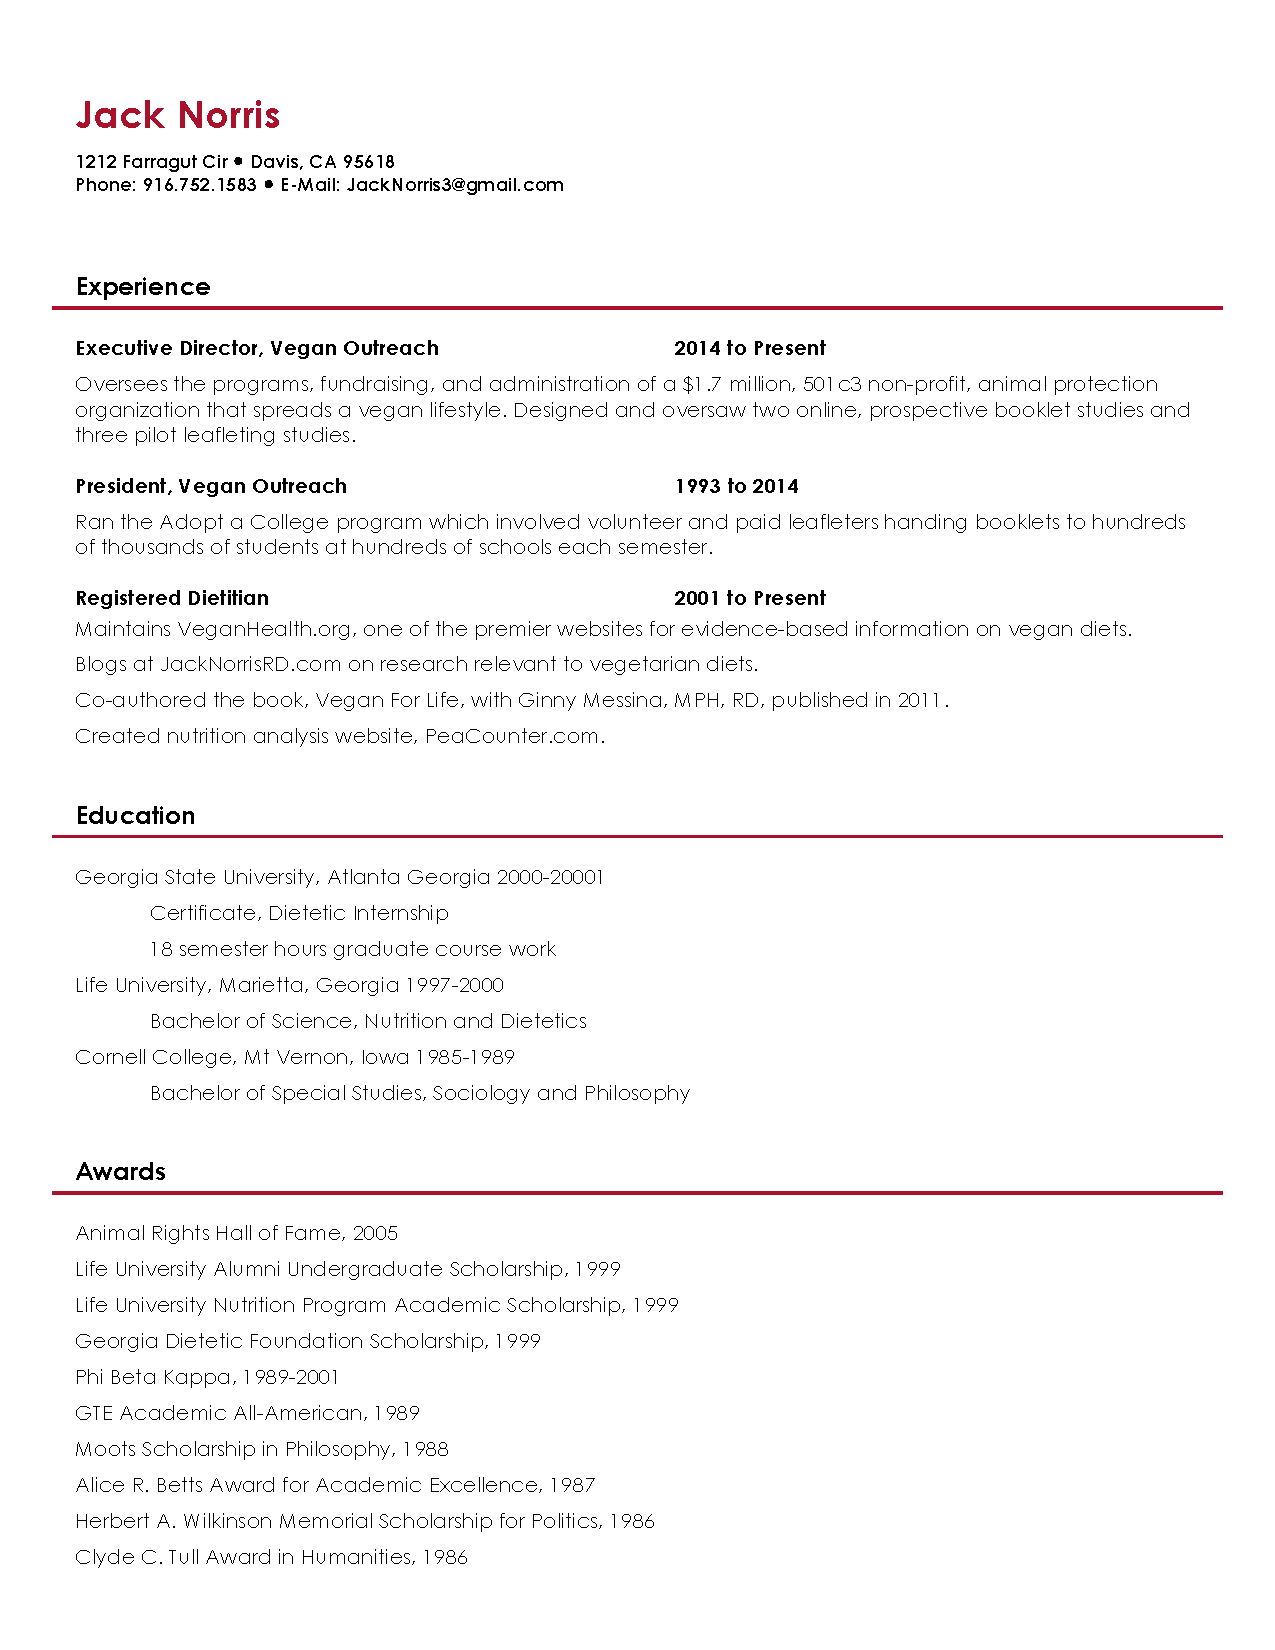
\includepdf[pages={-}]{resumes/jack_norris_cv.pdf}
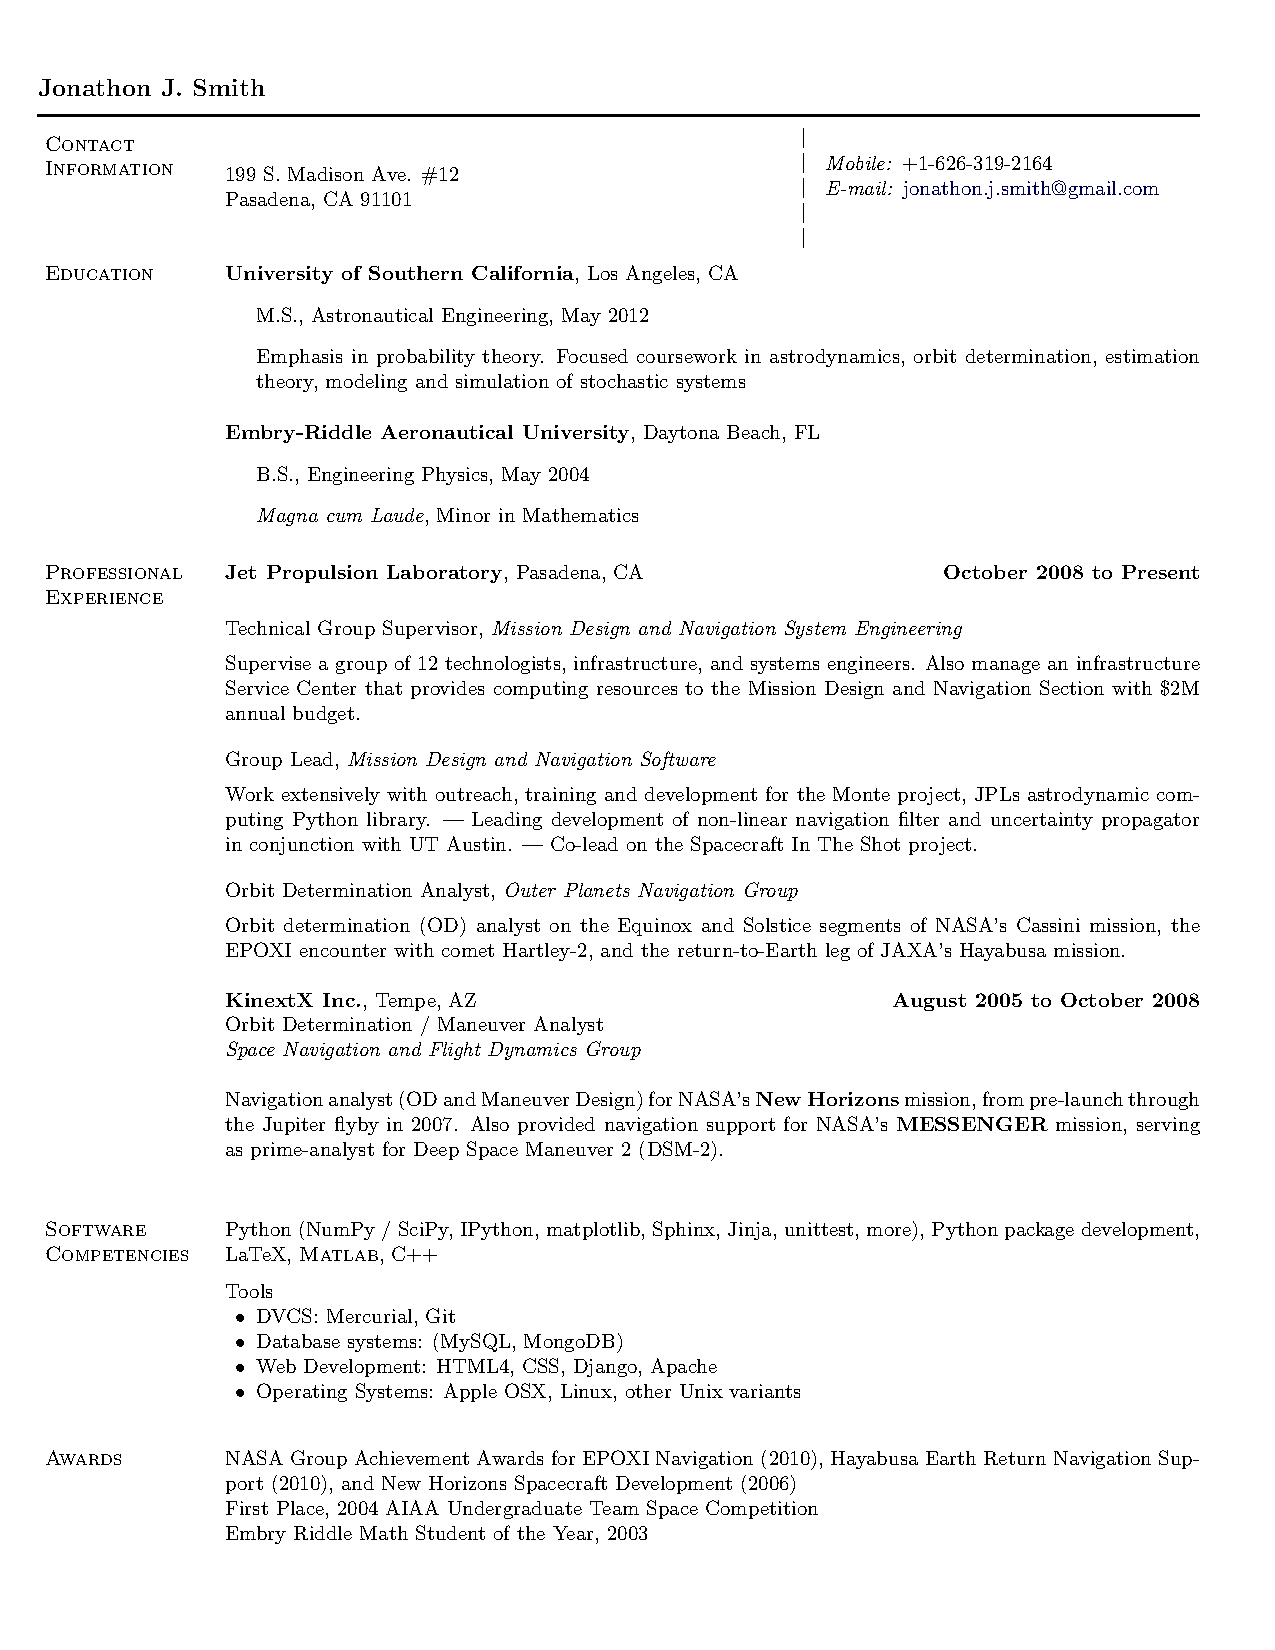
\includepdf[pages={-}]{resumes/jonathon_smith_cv.pdf}
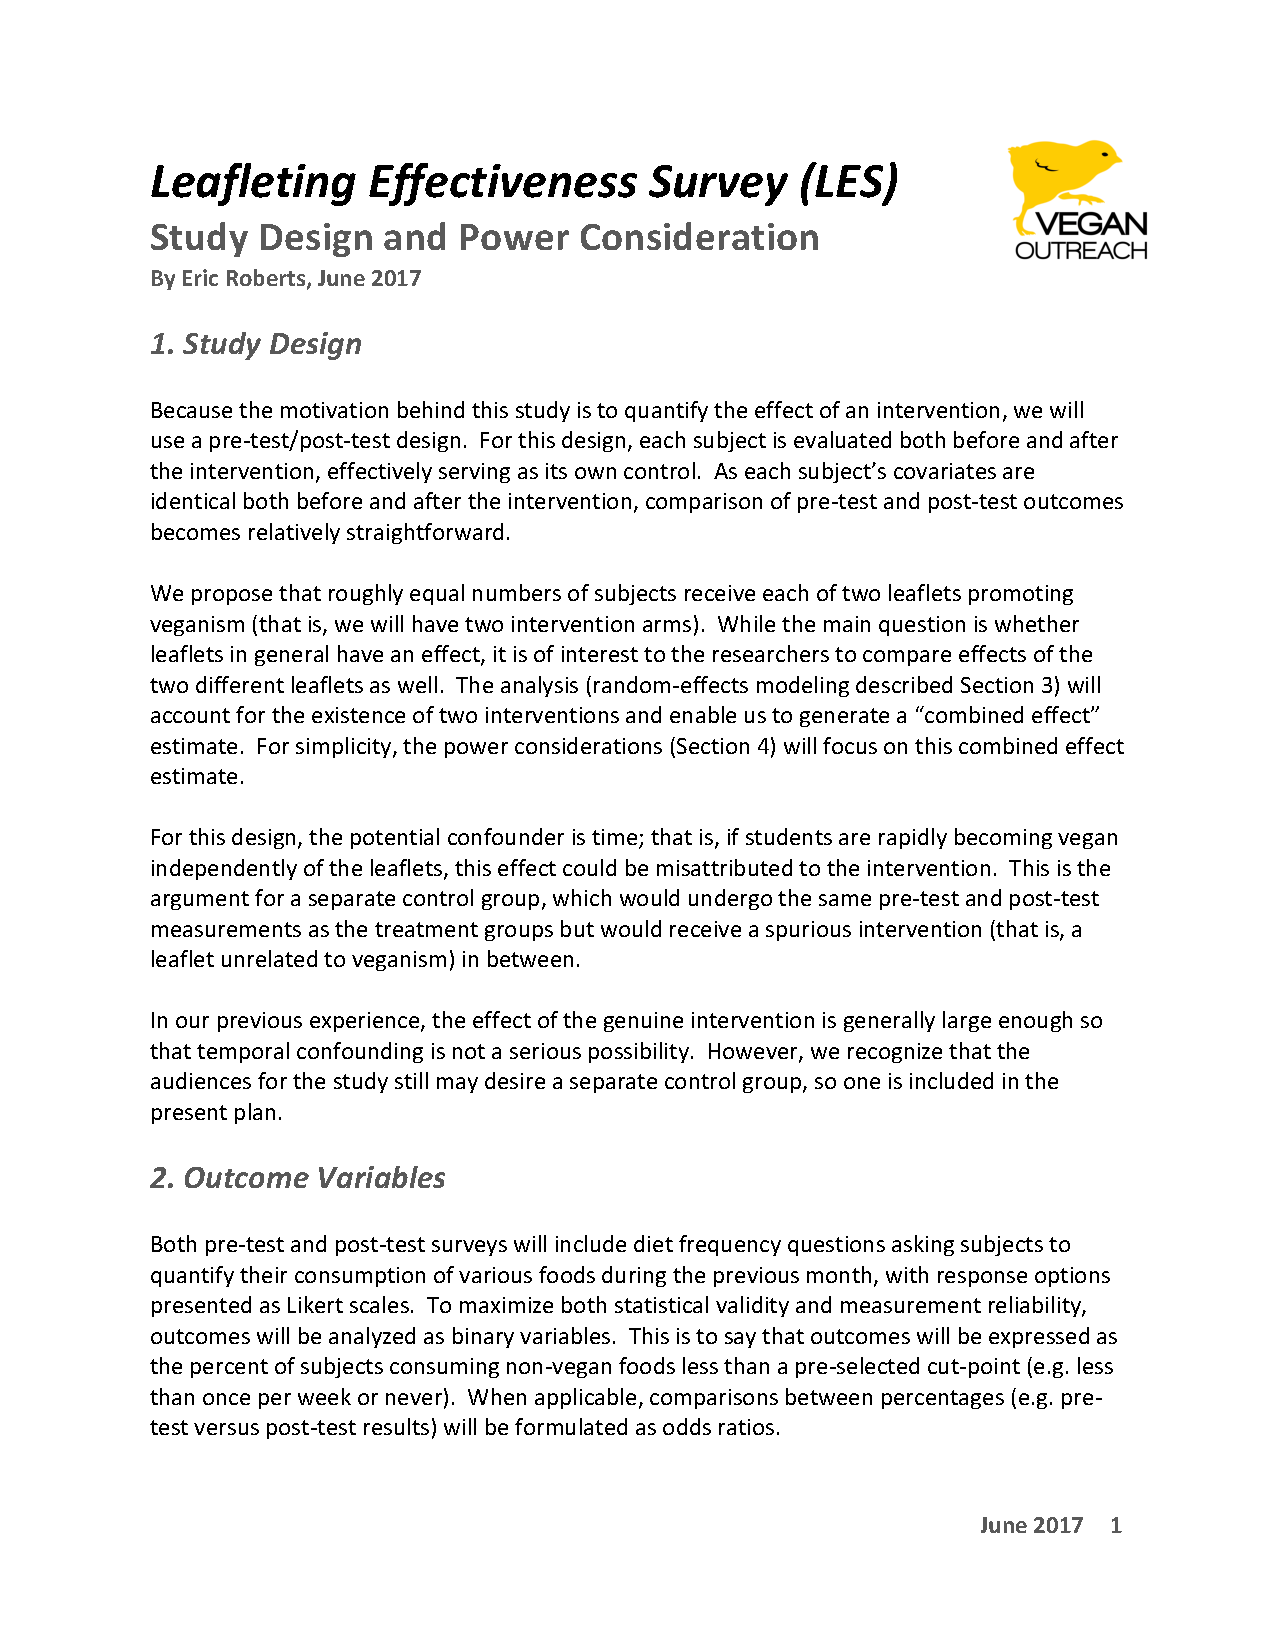
\includepdf[pages={-}]{../reference/VO_les_2017_methods.pdf}

\end{document}  
